In recent years, there has been a growth of interest in data visualization technologies for human-assisted data analysis using systems such as Polaris~\cite{Stolte:2008} and Spotfire~\cite{Ahlberg:1996}. While computers can provide high-speed and high-volume data processing, humans have domain knowledge and the ability to process data in parallel, notably by using our visual systems. Most importantly, humans provide the definition of what is valuable in an analysis. Accordingly, human/computer analytic systems are essential to extracting knowledge of value to humans and their societies from the large amounts of data being generated today.


\subsection{Interactivity}
Visualization systems are most effective when they are interactive, thereby allowing a user to explore data and connect it to their domain knowledge and sense of what is important without breaking cognitive flow. In recent years, a number of such systems have been developed, both by the academic community and by the commercial sector. Exploration of data consists not only in creating visual displays, but also in creating and modifying domain-specific computations. Consequently, most data visualization systems include facilities for defining such calculations as part of the data model being analyzed. The most effective systems allow users to define these calculations as part of the analytic interaction, which permits the user to stay in the flow of analysis~\cite{Morton:2012}.

During the analytic process, a user may discover that parts of the data are not yet suitable for analysis. Solutions to this problem are often provided by data preparation tools external to the visual analysis environment, which requires the user to break their analytic flow, launch another tool and reprocess their data before returning to their analysis. If the user does not own this process (\eg it is the responsibility of another department), then there can be significant delays (including ``never.'') More subtly, the result of updated external processing may not be compatible with the user's existing work, which can lead to more time lost reconciling the new data model with the existing analysis.

From the user's perspective, the boundary between preparation and analysis is not nearly so clean cut. Bad data is often discovered using visual analysis techniques (e.g. histograms or scatter plots) and it is most natural for the user to ``clean what she sees'' instead of switching to a second tool. This leads to an ``adaptive'' process whereby users will prefer leveraging existing tools in the analytics environment (no matter how well suited to the task) over switching to another application. Thus a well-designed interactive visual analysis environment will provide tools that enable users to perform such cleaning tasks as interactively as possible.

\subsubsection{Functions}
While the existing standards for query languages are helpful for defining a core set of row-level functions, there are many useful functions beyond the standards that are only explicitly supported by a subset of RDBMSes, often with different names. And even when a database does not provide an implementation of a particular function, it is usually possible to generate it as an inline combination of existing functionality. The calculation languages of visualization systems can thus be designed to provide a \textit{lingua franca} that tames this Babel of dialects by providing a common syntax for as many of these functions as possible.

\subsection{\dateparse}
The focus of this work is the usability of one such function from our visualization system that we will call \dateparse.

\subsubsection{	Scalar Dates}


The SQL-99 standard defines three temporal scalar types: \texttt{DATE}, \texttt{TIMESTAMP} and \texttt{TIME}. They are typically implemented as fixed-point types containing an offset from some epoch (\eg Julian Days.) This makes them compact to store using column store coompression techniques such as those in C-Store~\cite{Stonebraker:2005} and MonetDB/X100~\cite{Zukowski:2006}, and further allows some temporal operations to be implemented very efficiently using simple arithmetic. Thus from the RDBMS perspective, representing dates in scalar form provides  benefits for users, both in terms of available operations and query performance.

\begin{figure}[ht]
\centering
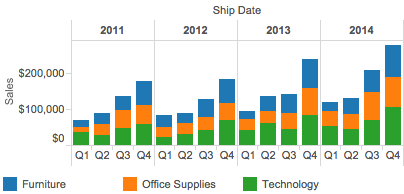
\includegraphics[width=\columnwidth]{figures/FigureI1}
\caption{Categorical Date Scalars.}
\label{fig:I1}
\end{figure}


Our visualization system models the first two of these SQL-99 types natively; the third (pure time) is folded into \texttt{TIMESTAMP} by appending it to a fixed date of \texttt{1899-12-30} (a convention derived from Microsoft Excel). From the analytic perspective, date types are dimensional (\ie independent variables) and can be used as either \textit{categorical} (simply ordered) or \textit{quantitative} (ordered with a distance metric) fields.

Categorical dates have a natural hierarchy associated with them generated by calendar \textit{binning}. The visualization in Figure \ref{fig:I1} shows an example of a bar chart employing binned categorical dates in a year/quarter hierarchy.

\begin{figure}[ht]
\centering
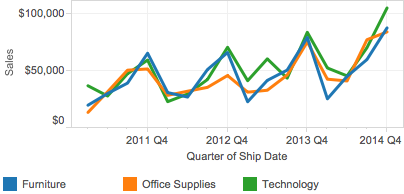
\includegraphics[width=\columnwidth]{figures/FigureI2}
\caption{Quantitative Date Scalars.}
\label{fig:I2}
\end{figure}



Quantitative dates are typically used for time series on an axis that maps the underlying distance measure to display pixel distance. The quantitative analog to categorical binning is \textit{truncation} whereby all the dates in a bin are represented by the first date in the bin. Truncation accurately preserves the distance semantics while enabling roll-up to coarser levels of detail. The visualization in Figure \ref{fig:I2} shows the same sales data in a time series rolled up to the quarter level.

These types of visualizations are difficult to specify with simple categorical string representations of dates. Thus the conversion of unparsed strings to date scalars is also an important component of data modeling for analytics.


\subsubsection{Parsing}
This parsing of date representations is one of the oldest data preparation problems we have observed. A common version of this problem is how to convert columns of integers of the form \texttt{yyyyMMdd} to date scalars. Naive users often solve this problem by converting the integer to a string and performing some locale-dependent string operations before casting the string back to a date. Unfortunately, this approach has a number of problems:
\begin{itemize}
\item String operations are notoriously slow compared to scalar operations (typically 10-100x slower in modern RDBMSes)
\item Default parsing of date formats is locale-dependent, and may not work when the analysis is shared across an international organization (\eg between the US and European offices)
\item The parsing code was hard to understand and maintain because it used a verbose, general-purpose string-handling syntax instead of a specialized domain language.
\end{itemize}

And this is but a single date format. Our studies of online data collections suggest that there are hundreds of distinct temporal date formats in user data sets. Some are common, but others can be quite idiosyncratic. Table 1 shows a selection of unusual date formats found in our test data. The first example shows a time zone in the middle of the date and a year after the time; the second shows a leading unmatched bracket and a colon between the date and time components; the third shows confusion between the seconds' decimal point and the time part delimiter; the fourth shows a two digit year apostrophe on a four digit year and the fifth shows a dash separating the date and time components.



\begin{table}[ht]
\centering
%\begin{tabular}{ |l|l|l| }
\begin{tabular}{|p{0.498\linewidth}| p{0.485\linewidth}|}
\hline
\centering
\textbf{ICU Format} & \textbf{Example}\\ \hline
\scriptsize{EEE MMM dd HH:mm:ss zzz yyyy} & \scriptsize{Fri Apr 01 02:09:27 EDT 2011}\\ \hline
\scriptsize{[dd/MMM/yyyy:HH:mm:ss} & \scriptsize{[10/Aug/2014:09:30:40}\\ \hline
\scriptsize{dd-MMM-yy hh.mm.ss.SSSSSS a} & \scriptsize{01-OCT-13 01.09.00.000000 PM}\\ \hline
\scriptsize{MM ''yyyy} & \scriptsize{01 '2013}\\ \hline
\scriptsize{MM/dd/yyyy - HH:mm} & \scriptsize{04/09/2014 - 23:47}\\ \hline
\end{tabular}
\label{tab:dateformats}
\caption{Unusual Date Formats.}
\end{table}


Our first attempt to help users with this problem was to add a new function to the the calculation language called \dateparse. This function would take a string column and convert it to a datetime using a special purpose domain language for describing dates. Such functions exist in a number of databases (\eg MySQL, Oracle and Postgres), so it was a natural addition to the function library.

We chose the date parsing syntax defined by the International Components for Unicode (or ICU) project~\cite{ICU} for the common domain language because it mirrored what was already available in our code base, and translating this syntax into the formats used by various database vendors was relatively painless. There are a few patches of non-overlapping functionality, but they tend to be obscure and we provide warnings when functionality is missing.

\subsubsection{	Usability}
After providing this new function to our user base, we waited a few months and then investigated how it was being applied in a free, cloud-based version of the system. We found that although there were a number of new calculations using \dateparse, the error rate for the domain language syntax was about 15\%. \dateparse was capable of solving the problem, and some users were able to discover it, but the syntax did not appear to be easy to use reliably.

\subsection{Automated Format Extraction}
One solution to this problem might have been to design a graphical environment that enabled users to construct valid patterns. This would have involved a substantial development effort with no guarantee that the result would be correct if the user misunderstood the environment. Instead, we have developed two algorithms for automating the derivation of the format string, each of which uses a different machine learning technique. Both algorithms result in over 90\% parsing accuracy -- and 100\% syntactic correctness because they are machine generated.

% vidya: this probably should be its own section
% hawkfish: Not sure it is big enough, but I can see the logic.

\subsection{Related Work}
Data preparation has been considered an analytic bottleneck since at least the description of the Potter's Wheel system~\cite{Raman:2001}. Since then, several other interactive data preparation systems have been proposed, including Data Wrangler~\cite{Kandel:2011} and Google Refine~\cite{Refine}. While effective, these systems all make assumptions about possible date formats, which we suggest are too restrictive for real world data.

Various approaches have been described for deriving regular expressions, and a good overview is provided by Li et al. in their paper on the ReLIE system for deriving regular expressions given a starting expression provided by a domain expert~\cite{Li:2008}. The Minimum Descriptive Length technique first described in Rissanen~\cite{Rissanen:1978} was used in~\cite{Raman:2001} to generate regular expressions. 

Related work on parsing languages, outlier detection??

\subsection{Overview}
The rest of this paper is organized as follows: The next section introduces the parameters of the problem space. The following two sections describe the two different algorithms, one using Minimum Descriptive Length and the other using Natural Language Processing. In section 5, we evaluate the algorithms on a corpus of 30K columns, both by sampling the outputs manually and then by using the algorithms to validate each other. We then discuss future work in section 6 and conclude in section 7.
